\documentclass[UTF8]{ctexart}
%\setcounter{secnumdepth}{0}
\usepackage{amsmath}
\usepackage{fancyhdr}
\usepackage{enumitem}
\usepackage{geometry}
\usepackage{graphicx}
\usepackage{titlesec}
\usepackage{multirow}
\usepackage{caption}
\usepackage{wrapfig}
\usepackage{multirow}
\usepackage{wrapfig}
\usepackage[justification=centering]{caption}
\geometry{left=3.18cm, right=3.18cm, top=2cm, bottom=2cm}
\pagestyle{empty}
\titleformat{\subsubsection}[runin]{\normalfont\large\bfseries}{\thesubsection}{1em}{}
% \newcommand{\setParDis}{\setlength {\parskip} {-15pt} }
% \newcommand{\setParDef}{\setlength {\parskip} {0pt} }
\pagestyle{plain}
\captionsetup{font={small}}
\renewcommand{\thefootnote}{}
% \renewcommand\thetable{\alph{表格}}

\begin{document}
    \title{植物生理学实验报告\\综合实验:多效唑处理对小麦不同生理指标影响}
    \author{李睿 \ \ 生物科学201903 \ \ 201900886}
    \date{\today{}}
    \maketitle
    \newpage

    \tableofcontents
    \newpage

    % \begin{abstract}
    % \end{abstract}
    \textbf{摘要:}多效唑作为一种植物生长延缓剂,有着矮化植株、增强植物抗逆性等作用。
    本实验测定了不同浓度多效唑处理下的小麦种子$\alpha$-淀粉酶活性、小麦幼苗形态、丙二醛含量、叶绿素含量和脯氨酸含量,
    结果表明多效唑可以增强小麦种子$\alpha$-淀粉酶活性、降低小麦幼苗的株高,降低幼苗中中丙二醛含量,提高脯氨酸的含量,对叶绿素含量的影响不明显。
    \\
    \indent \textbf{关键词:}多效唑、小麦、丙二醛、脯氨酸
    
    

   
    
    % %\begin{enumerate}[itemindent=1em]
    %     \begin{flushleft}
    %     \end{flushleft}
    % %\end{enumerate}


    \section{背景介绍}
    多效唑是一种植物生长延缓剂,在农业中被广泛使用。多效唑有拮抗赤霉素的作用,通过抑制赤霉素的生物合成而延缓植物生长。当赤霉素的合成被抑制时,细胞仍然进行分裂,但新生成的细胞不会伸长,从而使植物枝干长度减少。多效唑还可能诱导叶片气孔变小、叶片变厚、叶片颜色更深,并增加根系密度,从而使植物具有更好的耐受干旱的能力。
    \\
    \indent 本实验测定了小麦种子和幼苗的多种生理指标,包括$\alpha$-淀粉酶活性、小麦幼苗形态、幼苗的丙二醛、叶绿素和脯氨酸含量。从这些指标中探究多效唑浸种对小麦抗逆性的影响。


    % \begin{wrapfigure}[5]{l}{20em} % 纵向8行,图片靠右,宽度12.5em
    %     \begin{center}
    %         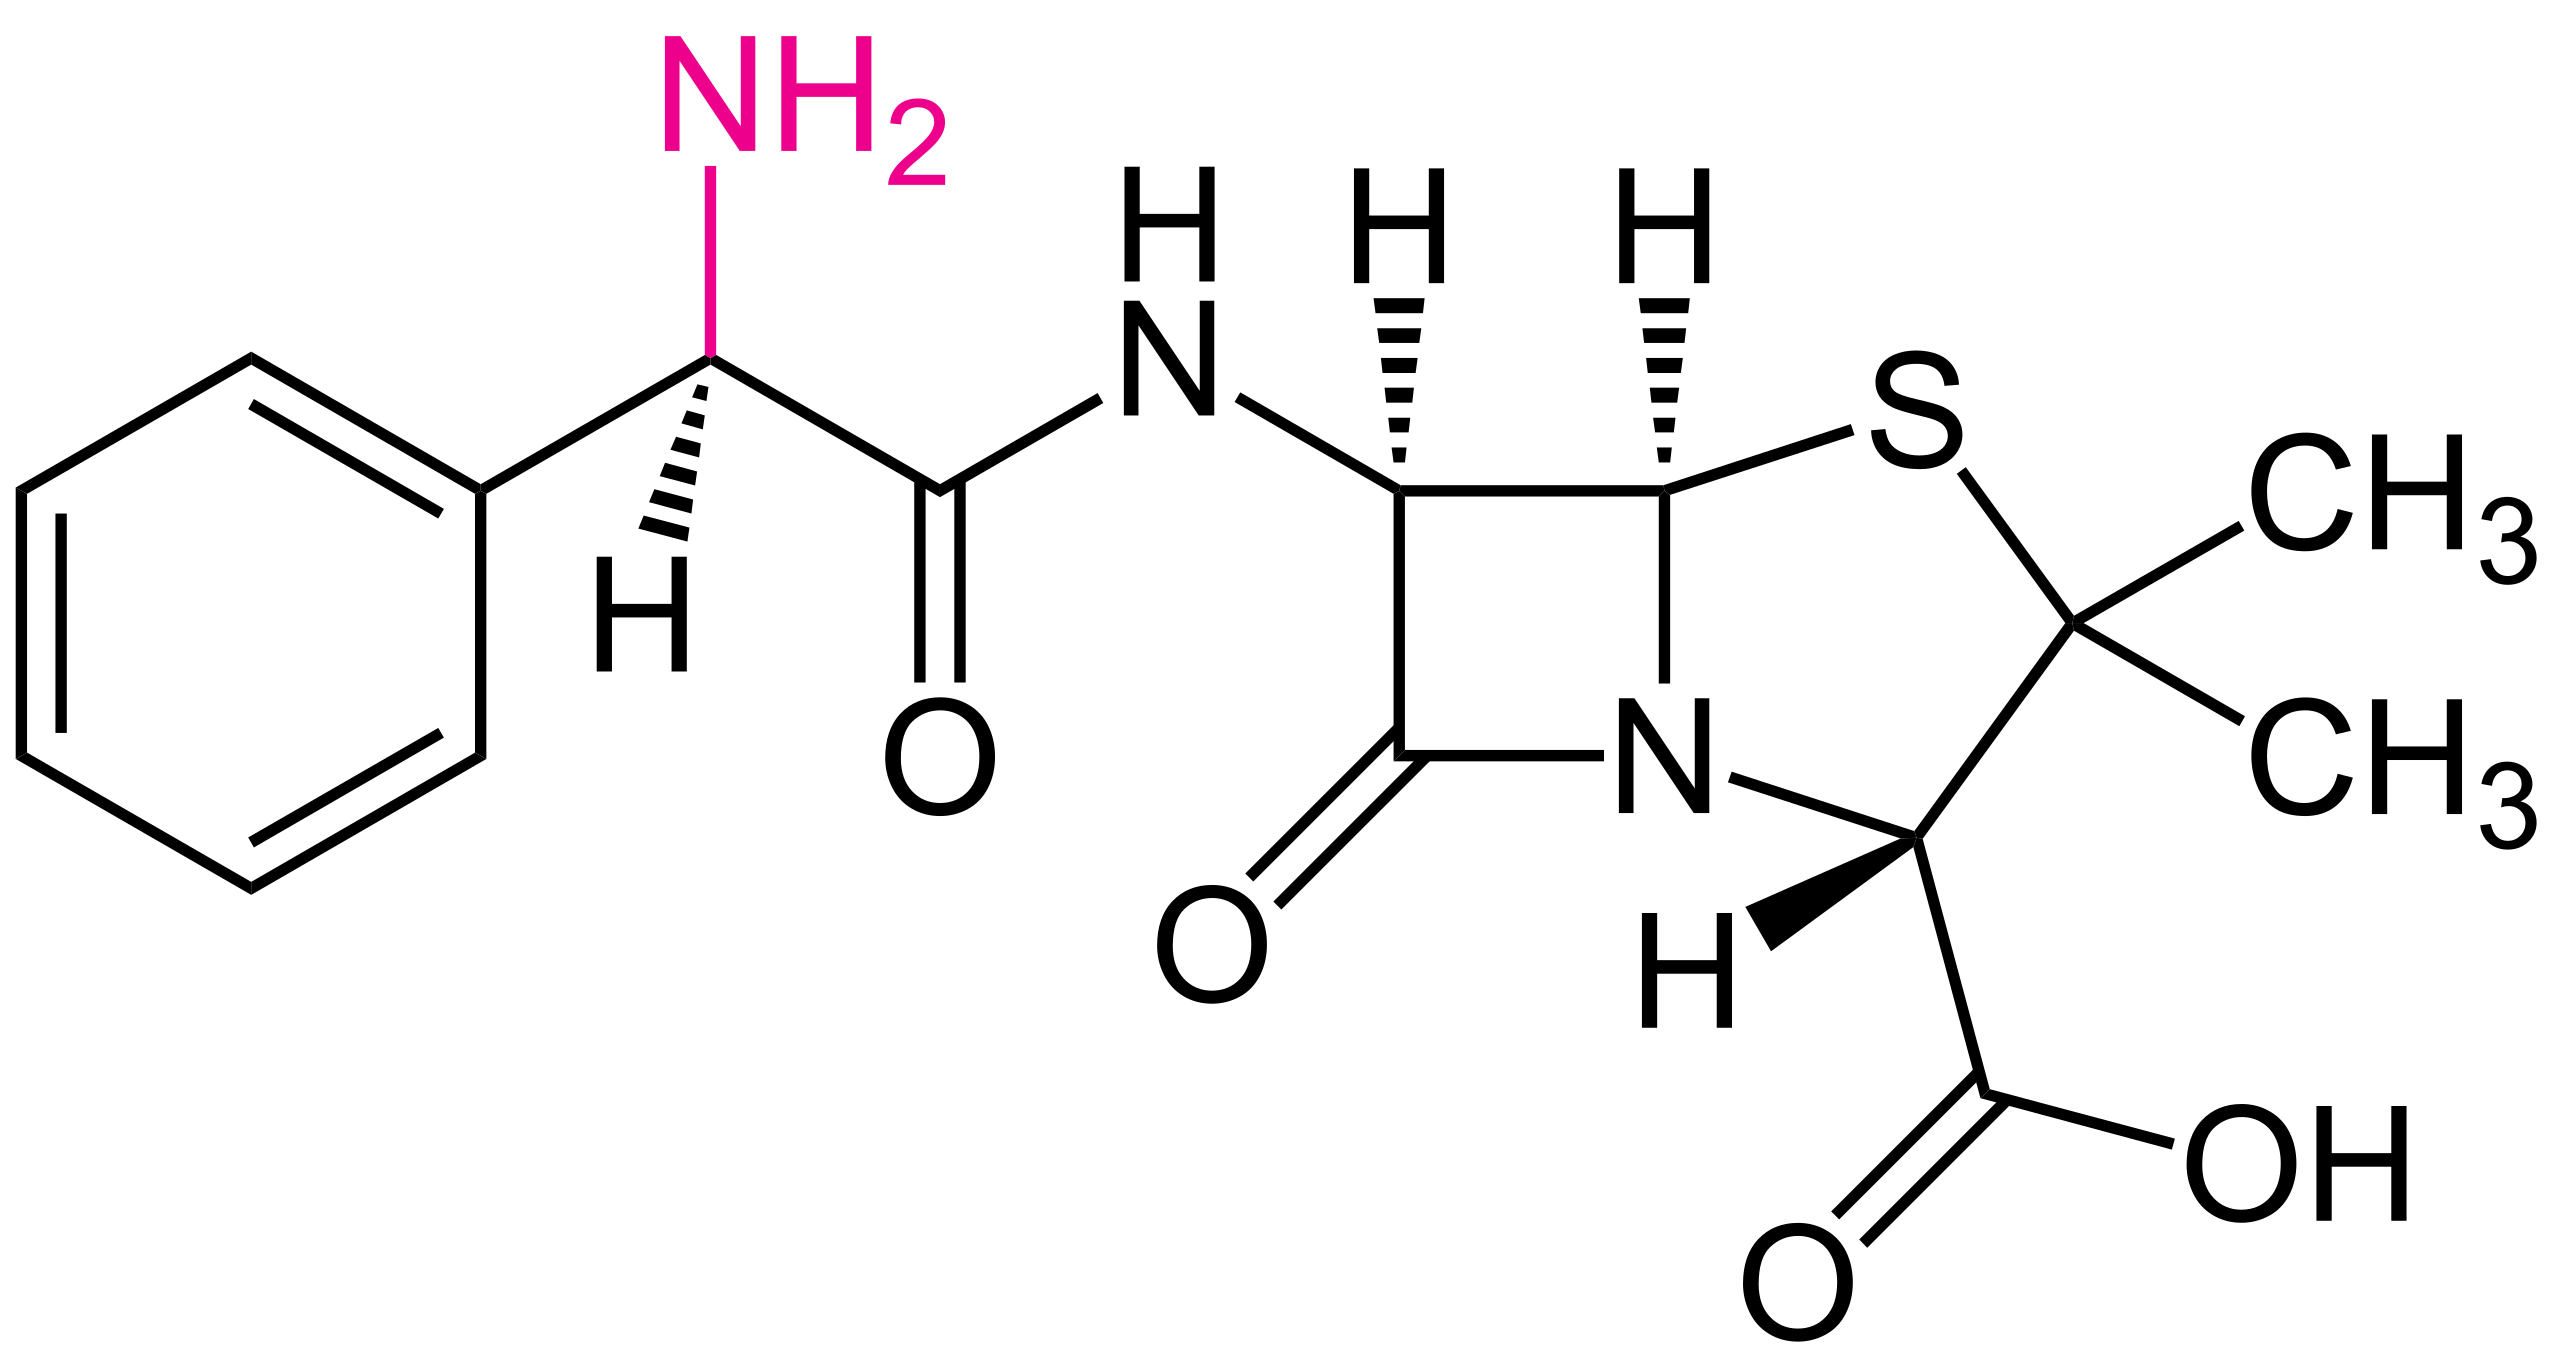
\includegraphics[scale=0.05]{Ampicillin_with_amine_highlighted.png}
    %         \caption{氨苄青霉素与青霉素G相比在与苯环相连的$\alpha$碳上引入了氨基,使其耐酸并更容易进入细菌细胞膜。}
    %         \label{fig:label}
    %     \end{center}
    % \end{wrapfigure}
    % \indent 氨苄青霉素是青霉素G侧链羧基的$\alpha$位引入氨基,改变了它的极性,使其更容易透过细菌细胞膜。同时它具有耐酸的特征,避免了天然青霉素不宜内服的缺点,为临床给药提供了很大的方便,在临床上得以广泛应用。
    
    
    
    \section{材料和方法}

    \subsection{小麦种子的处理}
    \subsubsection*{选种及种子灭菌}
    选取籽粒饱满、大小一致、无病虫害、胚部无损伤的小麦种子,用1\% NaClO消毒
    浸泡30min,然后用蒸馏水冲洗3-5次。
    \subsubsection*{浸种}
    将灭菌后的种子放入20$^{\circ}$C的蒸馏水中浸泡8h,再将实验组种子放入50mg/ml、100mg/ml的多效唑
    浸提液中浸种16h,温度为20$^{\circ}$C,对照同条件相同。
    \subsubsection*{培养}
    取直径为9cm的培养皿,垫上已湿润的滤纸,并排除纸间气泡。选取饱满、露白一致、大小一致的在室温(20$^{\circ}$C)下
    已浸种催芽24h的小麦种子,30粒腹沟朝下均匀放在培养皿中,每个处理设置2个重复,分别加入蒸馏水,使小麦种子
    保持湿润状态。每天定时进行湿度(85\%RH)、温度(28$^{\circ}$C)、光照(40\%)的管理,在培养过程中分别补加水使滤纸保持湿润。
    
    \subsection{小麦种子$\alpha$-淀粉酶活性测定}
    \subsubsection*{麦芽糖标准曲线制作}
    取7支干净的具塞刻度试管,按表1加入试剂摇匀,沸水浴5min,取出后流水冷却,加蒸馏水定容至10mL。用分光光度计测定吸光值A$_{540}$。以麦芽糖含量为横坐标,吸光度值A$_{540}$为纵坐标,绘制标准曲线。
    \subsubsection*{酶液制备}
    取0.5 g小麦种子(还未露白的为佳),研钵中加少量的石英砂和2 mL柠檬酸缓冲液(pH=5.6),研磨至匀浆。将匀浆倒入离心管中,再用6 mL柠檬酸缓冲液分次将残渣洗入离心管,室温下放置提取20 min,每隔数分钟搅动1次,使其充分提取。3000 r/min离心10 min,上清液倒入25 mL容量瓶中,加柠檬酸缓冲液定容至刻度,摇匀,即为淀粉酶原液。
    \subsubsection*{酶活测定}
    取3支干净的刻度试管,按下表顺序加入试剂及相应处理后,分光光度计测定吸光度A$_{540}$,1号管做空白参比,2、3号管的值取平均值,在标准曲线上查出相应的麦芽糖含量(mg),即求得$\alpha$-淀粉酶活力(U),再根据公式计算出$\alpha$-淀粉酶比活力(mg/g)。
    \begin{table}[h]
        \centering
        % \renewcommand{\arraystretch}{1.3}
        \setlength{\abovecaptionskip}{0.cm}
        \caption{淀粉酶活力测定方法}
        \resizebox{\textwidth}{!}{%
        \begin{tabular}{lccc}
        \hline
        \multicolumn{1}{c}{\multirow{2}{*}{\textbf{试剂及处理方式}}} & \multicolumn{3}{c}{\textbf{试管编号}} \\ \cline{2-4} 
        \multicolumn{1}{c}{}               & 1           & 2   & 3   \\ \hline
        淀粉酶原液(mL)                          & 柠檬酸缓冲液(0.5) & 0.5 & 0.5 \\
        70℃水浴15 min,取出后流水冷却,钝化$\beta$-淀粉酶;       & √           & √   & √   \\
        40 ℃恒温水浴中保温10 min                  & √           & √   & √   \\
        1\%淀粉溶液(mL)                        & 0.5         & 0.5 & 0.5 \\
        40℃恒温水浴中保温5 min                    & √           & √   & √   \\
        3,5-二硝基水杨酸(mL)                     & 1           & 1   & 1   \\
        摇匀,沸水水浴5 min,取出后流水冷却,加蒸馏水定容至10 mL; & √           & √   & √   \\ \hline
        \end{tabular}%
        }
    \end{table}


    \subsection{小麦幼苗形态测定}
    从每个培养皿中随机取出10株生长2周左右的小麦幼苗,用直尺测量其根长及芽长:根长测量随机选取材料的主根根长,取平均值;芽长从选取的幼苗发芽底部开始测量,取平均值;根数测量包括主根在内的根数。

    \subsection{丙二醛含量测定}
    \subsubsection*{MDA提取}
    取叶片0.5 g左右,置于研钵,加入2 mL 10\% TCA和少许石英砂,研磨成匀浆,加入6 mL 10\% TCA继续研磨,匀浆转入离心管,在3000 r/min下离心10 min,上清即为提取液(可转移上清到新的10 mL 离心管中,记录提取液总体积)。
    \subsubsection*{显色测定}
    10 mL刻度试管4只,3支各加入(三个处理组小麦)提取液3 mL,另1只加入蒸馏水3 mL,各加入0.5\% TBA溶液3 mL,摇匀,沸水浴中煮沸10 min,立即在冷水中冷却。以空白为参比,测定吸光度值(450、532、600 nm)。

    \subsection{叶绿素含量测定}
    称取小麦幼苗叶片0.2 g,加入适量碳酸钙粉及2 mL 95\%的乙醇,研磨成无大组织碎片后再加5 mL 95\%乙醇,
    继续研磨至匀浆,静置5 min,转入离心管,于3000 r/min离心10 min,上清转移到25 mL的容量瓶; 
    再用6 mL 95\%乙醇冲洗研钵、研棒及残渣后再离心,上清转移至容量瓶,95\%乙醇定容至25 mL,摇匀。
    以95\%乙醇溶液做空白参比调零,在波长663、645 nm下测吸光度值。


    \subsection{脯氨酸含量测定}
    \subsubsection*{脯氨酸的提取}
    称取各组材料0.5 g左右放入研钵中,加少量80\%乙醇和石英砂,研磨成匀浆,转入50 mL离心管中(匀浆总体积10 mL左右),摇匀,盖紧,80$^{\circ}$C水浴20 min。
    \subsubsection*{脱色与去杂}
    向大离心管中加入活性炭0.25 g和人造沸石1 g左右,剧烈摇荡5 min左右,在3000 r/min下离心10 min,上清液转到25 mL容量瓶中, 加入80\%乙醇清洗离心管2-3次,在3000 r/min下离心10 min,合并上清,用80\%乙醇定容到刻度。
    \subsubsection*{显色反应}
    吸取提取液2 mL、冰醋酸、酸性茚三酮各2 mL加入具塞刻度试管中,加塞沸水浴15 min,冷却后比色测定。
    \subsubsection*{比色测定}
    用80\%乙醇做空白参比,在515 nm下测吸光度值。
    \subsubsection*{标准曲线制作}
    取100 μg/mL脯氨酸标准液2 ml,加水稀释至10 ml,脯氨酸标准液浓度20 μg/mL。
    按表2配制分别含脯氨酸0、2、4、6、8、12、16、20 μg/mL 的溶液,加入各试剂混匀后沸水浴15 min,冷却后,用80\%乙醇做空白参比,在515 nm下测吸光度值。 

    \begin{table}[]
        \centering
        \setlength{\abovecaptionskip}{0.cm}
        \caption{脯氨酸标准曲线配制}
        \begin{tabular}{lllllllll}
        \hline
        管号           & 0   & 1   & 2   & 3   & 4   & 5   & 6   & 7   \\ \hline
        脯氨酸浓度(ug/mL) & 0   & 2   & 4   & 6   & 8   & 12  & 16  & 20  \\
        脯氨酸标准液(mL)   & 0.0 & 0.2 & 0.4 & 0.6 & 0.8 & 1.2 & 1.6 & 2.0 \\
        80乙醇(mL)     & 2.0 & 1.8 & 1.6 & 1.4 & 1.2 & 0.8 & 0.4 & 0.0 \\
        冰醋酸(mL)      & 2.0 & 2.0 & 2.0 & 2.0 & 2.0 & 2.0 & 2.0 & 2.0 \\
        酸性茚三酮(mL)    & 2.0 & 2.0 & 2.0 & 2.0 & 2.0 & 2.0 & 2.0 & 2.0 \\
        吸光度A(515nm)  &     &     &     &     &     &     &     &     \\ \hline
        \end{tabular}
    \end{table}

    \section{结果}
    \subsection{多效唑处理使小麦种子淀粉酶活性增强}
    淀粉酶活力的大小与产生还原糖的量成正比。因此,实验采用麦芽糖制作标准曲线,用比色法测定淀粉生成的还原糖的量。以一定时间内生成的还原糖的量表示酶活力。$\alpha$-淀粉酶不耐热,在70℃保温15 min被钝化。本实验采用加热钝化$\beta$-淀粉酶,进而测定出$\alpha$-淀粉酶的活力。
    
    \begin{table}[h]
        \centering
        \setlength{\abovecaptionskip}{0.cm}
        \caption{麦芽糖标准曲线}
        % \resizebox{\textwidth}{!}{%
        \begin{tabular}{llllllll}
        \hline
        管号        & 1 & 2     & 3     & 4     & 5     & 6     & 7     \\ \hline
        麦芽糖含量(mL) & 0 & 0.1   & 0.3   & 0.5   & 0.7   & 0.9   & 1.0   \\
        吸光度A$_{540}$   & 0 & 0.090 & 0.353 & 0.669 & 0.936 & 1.173 & 1.234 \\ \hline
        \end{tabular}%
        % }
    \end{table}


    \begin{wrapfigure}[7]{r}{9cm}%靠文字内容的右侧
        \caption{麦芽糖标准曲线}
        \setlength{\abovecaptionskip}{0.cm}
        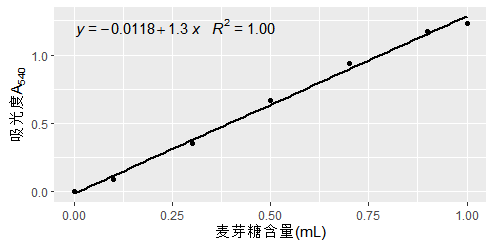
\includegraphics[scale=0.75]{maiyatang.png}
    \end{wrapfigure}


    \indent 淀粉酶包括$\alpha$-淀粉酶和$\beta$-淀粉酶。$\alpha$-淀粉酶能随机地作用于淀粉的非还原端,使其生成麦芽糖、麦芽三糖和糊精等还原糖,而使淀粉浆的粘度下降。生成的还原糖可以使3,5-二硝基水杨酸还原,生成棕红色的3-氨基-5-硝基水杨酸,该物质在540 nm处有最大吸收峰。    
    \\ \indent 经测定,一定浓度多效唑处理的种子淀粉酶活力增加,随着浓度的增大,增加效果越来越显著(50mg/mL处理: p-value = 0.2232, 100mg/mL处理: p-value = 0.0642, Student's\ \textit{t}检验)。
    \\ \indent 定义5 min内淀粉酶分解淀粉产生的麦芽糖的量为1个活力单位
    \begin{center}
    $\mbox{比活力(mg/g)} = \frac{m \times D}{M} $
    \\ $\mbox{m:麦芽糖含量(mg)}; \mbox{M:样品重量}; \mbox{D:酶液重量在反应系统中酶液的倍数}$
    \\
    \end{center}
    \ 
    \\ \indent 0mg/mL处理组酶活力为10.41,50mg/mL为13.88,100mg/mL处理组为18.36。

    \begin{table}[!h]
        \centering
        \setlength{\abovecaptionskip}{0.cm}
        \caption{淀粉酶活力}
        \begin{tabular}{lclclcl}
        \hline
        多效唑处理浓度(mg/L) & \multicolumn{2}{c}{0}             & \multicolumn{2}{c}{50}            & \multicolumn{2}{c}{100}          \\ \hline
        重量            & \multicolumn{2}{c}{0.48g}         & \multicolumn{2}{c}{0.54g}         & \multicolumn{2}{c}{0.49g}        \\
        吸光度A540       & \multicolumn{1}{l}{0.161} & 0.128 & \multicolumn{1}{l}{0.203} & 0.214 & \multicolumn{1}{l}{0.240} & 0.256 \\ \hline
        \end{tabular}
    \end{table}

    \subsection{多效唑处理使幼苗矮化和生根减少}
    多效唑通过抑制赤霉素的合成来抑制细胞伸长,对植物有着明显的矮化效果,并促进幼苗生根。本实验测定了0、50、100mg/mL的幼苗的芽长、根长和生根数。结果表明多效唑有缩短
    芽长和根长,减少生根数的效果。具体来说,50mg/ml、100mg/mL的多效唑处理显著降低了芽长(50mg/mL处理: p-value = 6.293e-13, 100mg/mL处理: p-value = 3.231e-07, Student's\ \textit{t}检验)。
    50mg/mL处理平均降低芽长4.98cm,100mg/mL处理平均降低芽长5.65cm。在浓度达到50mg/mL后,再增加多效唑浓度对植物的矮化效果不显著(p-value = 0.2142)。
    

    %有趣的是,100mg/mL处理的芽长的方差远远大于50mg/mL的处理组,
    %而在根长和生根数的测定中,50mg/mL和100mg/mL的方差几乎相同。在根长的测定中,50mg/mL处理平均降低根长4.84cm,100mg/mL处理平均降低根长4.94cm,二者效果几乎相同,说明根对高浓度的多效唑比芽不敏感,多效唑也显著降低了小麦种子的生根数。


    \begin{table}[!h]
        \centering
        \setlength{\abovecaptionskip}{0.cm}
        \caption{小麦幼苗形态}
        % \resizebox{\textwidth}{!}{%
        \begin{tabular}{llllllllllll}
        \hline
                &    & 1    & 2    & 3    & 4    & 5    & 6    & 7    & 8    & 9    & 10   \\ \hline
        100mg/L & 芽长 & 11.6 & 10.1 & 6.7  & 7.0  & 7.7  & 9.4  & 8.2  & 8.1  & 9.0  & 9.5  \\
                & 根长 & 21.1 & 23.7 & 18.1 & 18.2 & 14.7 & 23.8 & 19.4 & 23.5 & 21.1 & 20.5 \\
                & 根数 & 7    & 5    & 5    & 7    & 4    & 6    & 6    & 5    & 5    & 5    \\ \hline
        50mg/L  & 芽长 & 8.7  & 8.6  & 8.9  & 10.0 & 10.1 & 9.2  & 9.9  & 10   & 9.8  & 8.8  \\
                & 根长 & 16.0 & 21.2 & 19.4 & 20.4 & 24.0 & 23.1 & 23.5 & 21.2 & 17.5 & 18.8 \\
                & 根数 & 6    & 6    & 7    & 6    & 6    & 8    & 6    & 5    & 6    & 4    \\ \hline
        0mg/L   & 芽长 & 14.5 & 14.2 & 15.2 & 14.3 & 14.2 & 14.8 & 14.1 & 14.6 & 14.0 & 13.9 \\
                & 根长 & 25.5 & 24.2 & 26.2 & 25.2 & 27.0 & 24.5 & 24.6 & 24.8 & 25.4 & 26.1 \\
                & 根数 & 12   & 12   & 11   & 10   & 11   & 13   & 9    & 12   & 10   & 14   \\ \hline
        \end{tabular}%
        % }
    \end{table}

    

    \subsection{多效唑处理降低了小麦幼苗的丙二醛含量}
    植物在逆境胁迫或者衰老的过程中,由于自由基、活性氧的积累引起膜质过氧化,进一步导致蛋白质交联变性,引起细胞损伤或死亡。丙二醛为膜质过氧化的最终产物。因此,测定丙二醛含量,可以了解植物的膜质氧化伤害程度。
    在酸性和高温条件下,MDA可以与硫代巴比妥酸(TBA)反应生成红棕色的三甲氚,在532 nm处有最大吸收值,在600 nm处有最小吸收值。TBA可与可溶性糖反应,在450 nm有最大吸收值,但在532 nm处也有吸收,为消除影响,需通过公式排除干扰。
    \begin{center}
        $c(\mu mol/L) = 6.45 \times (A_{532} - A_{600}) - 0.56 \times A_{450} $
        \\ $MDA(\mu mol/g) = cV \times 10^{-3}/W$
        \\ $c(\mu mol/L): \mbox{提取液中MDA浓度}; V(mL):\mbox{提取液的总体积}; W(g):\mbox{样品的鲜重}$
    \end{center}
    
    本实验测定了不同浓度多效唑处理后的小麦幼苗的丙二醛含量,按上述公式计算,0,50,100mg/mL处理的幼苗丙二醛含量分别为9.13$\mu mol/g$,5.22$\mu mol/g$,6.31$\mu mol/g$。
    吸光度测定结果表明50mg/mL和100mg/mL的处理均能使幼苗中的丙二醛含量显著降低(50mg/mL处理: p-value = 0.05901, 100mg/mL处理: p-value = 0.05979, 配对\textit{t}检验)。
    与幼苗形态的结果不同,在50mg/mL浓度后继续增加多效唑的浓度,其降低丙二醛的效果仍有差异(p-value = 0.1139, 配对\textit{t}检验)。

    \begin{figure}[!h]
        \centering
        \caption{不同浓度多效唑处理后的丙二醛含量}
        \setlength{\abovecaptionskip}{0pt}
        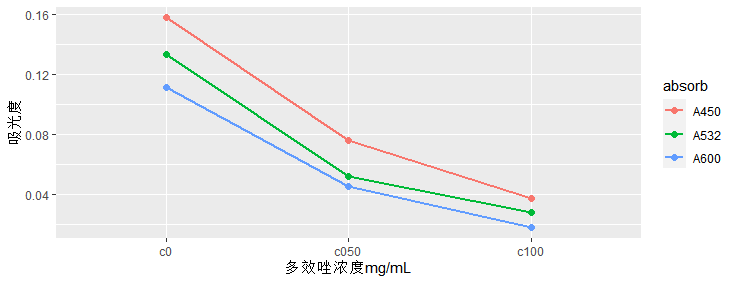
\includegraphics[scale=0.6]{bing.png}
    \end{figure}

    \begin{table}[!h]
        \centering
        \setlength{\abovecaptionskip}{0.cm}
        \caption{丙二醛含量}
        \begin{tabular}{llllll}
        \hline
        多效唑处理浓度(mg/L) & 重量    & 体积    & A450  & A532  & A600  \\ \hline
        0             & 0.52g & 7.6mL & 0.634 & 0.299 & 0.148 \\
        50            & 0.48g & 8.1mL & 0.519 & 0.201 & 0.108 \\
        100           & 0.51g & 7.4mL & 0.421 & 0.171 & 0.066 \\ \hline
        \end{tabular}
    \end{table}


    \subsection{多效唑处理提高了幼苗中脯氨酸含量}

    植物在干旱胁迫下会通过增加脯氨酸含量来增强植物对干旱胁迫的适应能力。
    脯氨酸可以调节植物的渗透式和增强蛋白质的亲水性而稳定蛋白质的结构和稳定细胞的结构与功能,以利于植物适应干旱胁迫。
    通过测定脯氨酸含量了解多效唑在抗逆性上的作用。
    采用80\%的乙醇提取叶片脯氨酸,脯氨酸在酸性条件下可与茚三酮加热后反应生成稳定的红色化合物,在515 nm下有最大吸收峰。通过分光光度法可以测定脯氨酸的含量。

    \begin{table}[!h]
        \centering
        \setlength{\abovecaptionskip}{0.cm}
        \caption{脯氨酸标准曲线}
        \begin{tabular}{lllllllll}
        \hline
        脯氨酸浓度($\mu$g/mL) & 0     & 2     & 4     & 6     & 8     & 12    & 16    & 20    \\ \hline
        A515         & 0.003 & 0.062 & 0.113 & 0.179 & 0.233 & 0.343 & 0.475 & 0.577 \\ \hline
        \end{tabular}
    \end{table}

    \begin{wrapfigure}[9]{r}{8.5cm}
        \centering
        \caption{脯氨酸标准曲线}
        \setlength{\abovecaptionskip}{0pt}
        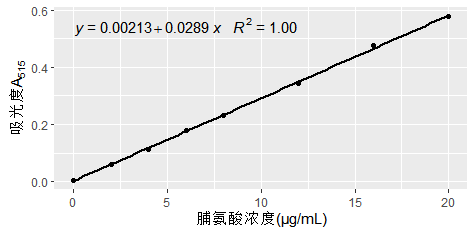
\includegraphics[scale=0.6]{pro.png}
    \end{wrapfigure}
    \begin{center}
        $\mbox{样品中脯氨酸含量}(\mu g/g \ FW)= \frac{C_{x} \times V}{FW} $
        \\ $C_{x}:\mbox{样品液的脯氨酸浓度}; V:\mbox{提取液总体积(mL)}; FW:\mbox{样品鲜重(g)}$
    \end{center}

    经测定,不同浓度多效唑处理的幼苗的脯氨酸含量分别为1.55$(\mu g/g \ FW)$,2.34$(\mu g/g \ FW)$,1.93$(\mu g/g \ FW)$,在50mg/mL的处理组中含量最高。多效唑可能会促进植物产生脯氨酸以适应
    逆境胁迫,在这种情况下,较低浓度的脯氨酸(50mg/mL)有对脯氨酸合成起促进作用,较高浓度(100mg/mL)又会抑制其合成。

    \begin{table}[!h]
        \centering
        \setlength{\abovecaptionskip}{0.cm}
        \caption{脯氨酸含量}
        \begin{tabular}{llll}
        \hline
        多效唑处理浓度(mg/L) & 0     & 50    & 100   \\ \hline
        幼苗重量(g)       & 0.51  & 0.50  & 0.49  \\
        A515          & 0.047 & 0.070 & 0.058 \\ \hline
        \end{tabular}
    \end{table}

    \subsection{多效唑处理未显著改变叶绿素含量}
    叶绿素含量是反应植物光合能力及营养状况的重要指标。叶绿素a在乙醇中对红光的吸收峰为663 nm,叶绿素b的吸收峰为645 nm。叶绿素对光的吸收服从朗白-比尔定律。因此,可以用分光光度计测定叶绿素提取液在663、645 nm波长下的吸光度,通过公式计算出叶绿素a、b及总叶绿素含量。
    \begin{center}
        $\mbox{叶绿素a}(mg/g)=(12.7A_{663}-2.69A_{645}) \times \frac{V}{1000 \times W} $
        $\mbox{叶绿素b}(mg/g)=(22.9A_{645}-6.48A_{663}) \times \frac{V}{1000 \times W} $
        $\mbox{总叶绿素}(mg/g)=(20.21A_{645}+8.02A_{663}) \times \frac{V}{1000 \times W} $
        \\ $A:\mbox{测定波长下的吸光度值}; V:\mbox{叶绿素提取液总体积(mL)}; W:\mbox{材料鲜重(g)}$
    \end{center}
    \begin{table}[!h]
        \centering
        \begin{tabular}{lllllll}
        \hline
        多效唑处理浓度(mg/L) & 幼苗重量(g) & A663 & A645 & 叶绿素a & 叶绿素b & 总叶绿素 \\ \hline
        0             & 0.2     & 1.17 & 0.40 & 1.72 & 0.47 & 2.19 \\
        50            & 0.18    & 1.04 & 0.43 & 1.68 & 0.70 & 2.37 \\
        100           & 0.19    & 1.32 & 0.49 & 2.03 & 0.66 & 2.69 \\ \hline
        \end{tabular}
    \end{table}

   
    \begin{figure}[!h]
        \centering
        \caption{不同浓度多效唑处理后的幼苗形态}
        \setlength{\abovecaptionskip}{0pt}
        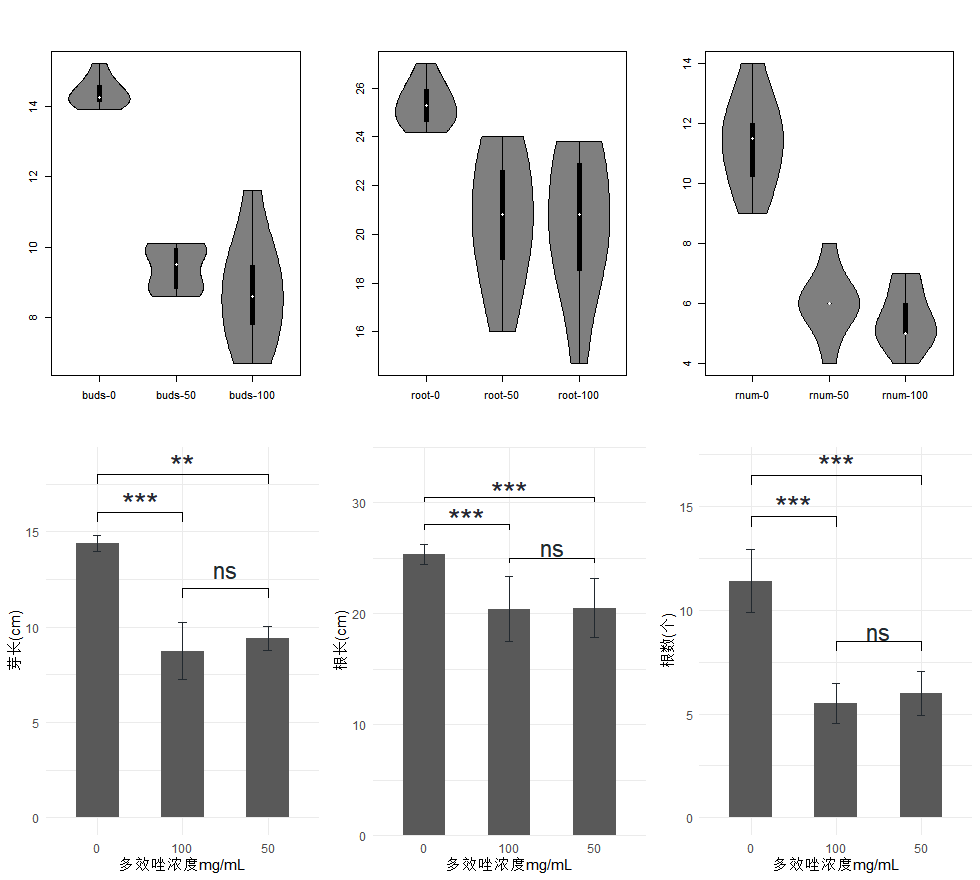
\includegraphics[scale=0.6]{comb.png}
    \end{figure}

    \section{讨论}
    \footnote{*latex和r源码见https://github.com/inspirewind/bioinfo-course/exp-plant-physiology}

\end{document}